\documentclass[11pt]{article}
\usepackage[textwidth=18.0cm, textheight=23.0cm, top=2.0cm]{geometry}
\usepackage{pst-all}
\usepackage{amssymb}
\usepackage{tikz}
\usepackage{underscore}\begin{document}
\pagestyle{empty}


ClassName: \underline{\textbf{Class_07.2bp-6}}
\par
BinSize: \underline{\textbf{100 × 100}}
\par
ReduceSize: \underline{\textbf{100 × 100}}
\par
TypeNum: \underline{\textbf{20}}
\par
Num: \underline{\textbf{20}}
\par
OutS: \underline{\textbf{40000}}
\par
InS: \underline{\textbf{32742}}
\par
Rate: \underline{\textbf{0.819}}
\par
UB: \underline{\textbf{4}}
\par
LB0: \underline{\textbf{4}}
\par
LB: \underline{\textbf{4}}
\par
LBWithCut: \underline{\textbf{4}}
\par
NodeCut: \underline{\textbf{0}}
\par
ExtendedNodeCnt: \underline{\textbf{1}}
\par
GenNodeCnt: \underline{\textbf{1}}
\par
PrimalNode: \underline{\textbf{0}}
\par
ColumnCount: \underline{\textbf{4}}
\par
TotalCutCount: \underline{\textbf{0}}
\par
RootCutCount: \underline{\textbf{0}}
\par
LPSolverCnt: \underline{\textbf{1}}
\par
PricingSolverCnt: \underline{\textbf{0}}
\par
BranchAndBoundNum: \underline{\textbf{1}}
\par
isOpt: \underline{\textbf{true}}
\par
TimeOnInitSolution: \underline{\textbf{600.000 s}}
\par
TimeOnPrimal: \underline{\textbf{0.000 s}}
\par
TimeOnPricing: \underline{\textbf{0.000 s}}
\par
TimeOnRmp: \underline{\textbf{0.063 s}}
\par
TotalTime: \underline{\textbf{600.328 s}}
\par
\newpage


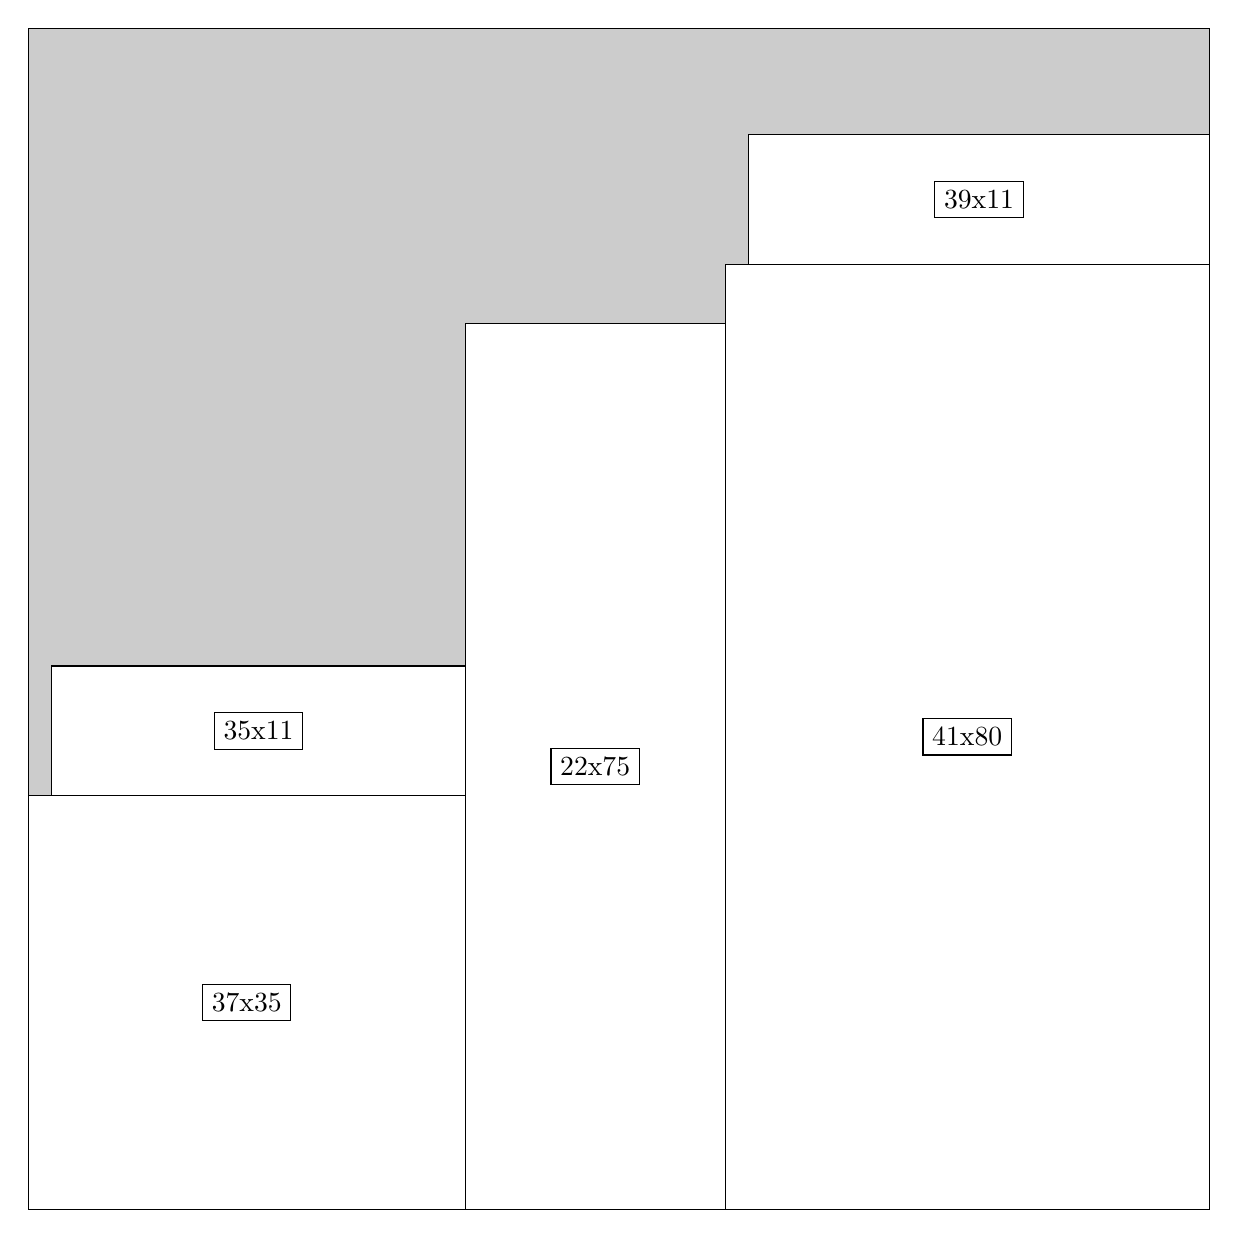
\begin{tikzpicture}[shorten >=1pt,scale=1.0,every node/.style={scale=1.0},->]
\tikzstyle{vertex}=[circle,fill=black!25,minimum size=14pt,inner sep=0pt]
\filldraw[fill=gray!40!white, draw=black] (0,0) rectangle (15.0,15.0);
\foreach \name/\x/\y/\w/\h in {41x80/8.85/0.0/6.1499999999999995/12.0,22x75/5.55/0.0/3.3/11.25,37x35/0.0/0.0/5.55/5.25,35x11/0.3/5.25/5.25/1.65,39x11/9.15/12.0/5.85/1.65}
\filldraw[fill=white!40!white, draw=black] (\x,\y) rectangle node[draw] (\name) {\name} ++(\w,\h);
\end{tikzpicture}


w =41 , h =80 , x =59 , y =0 , v =3280
\par
w =22 , h =75 , x =37 , y =0 , v =1650
\par
w =37 , h =35 , x =0 , y =0 , v =1295
\par
w =35 , h =11 , x =2 , y =35 , v =385
\par
w =39 , h =11 , x =61 , y =80 , v =429
\par
\newpage


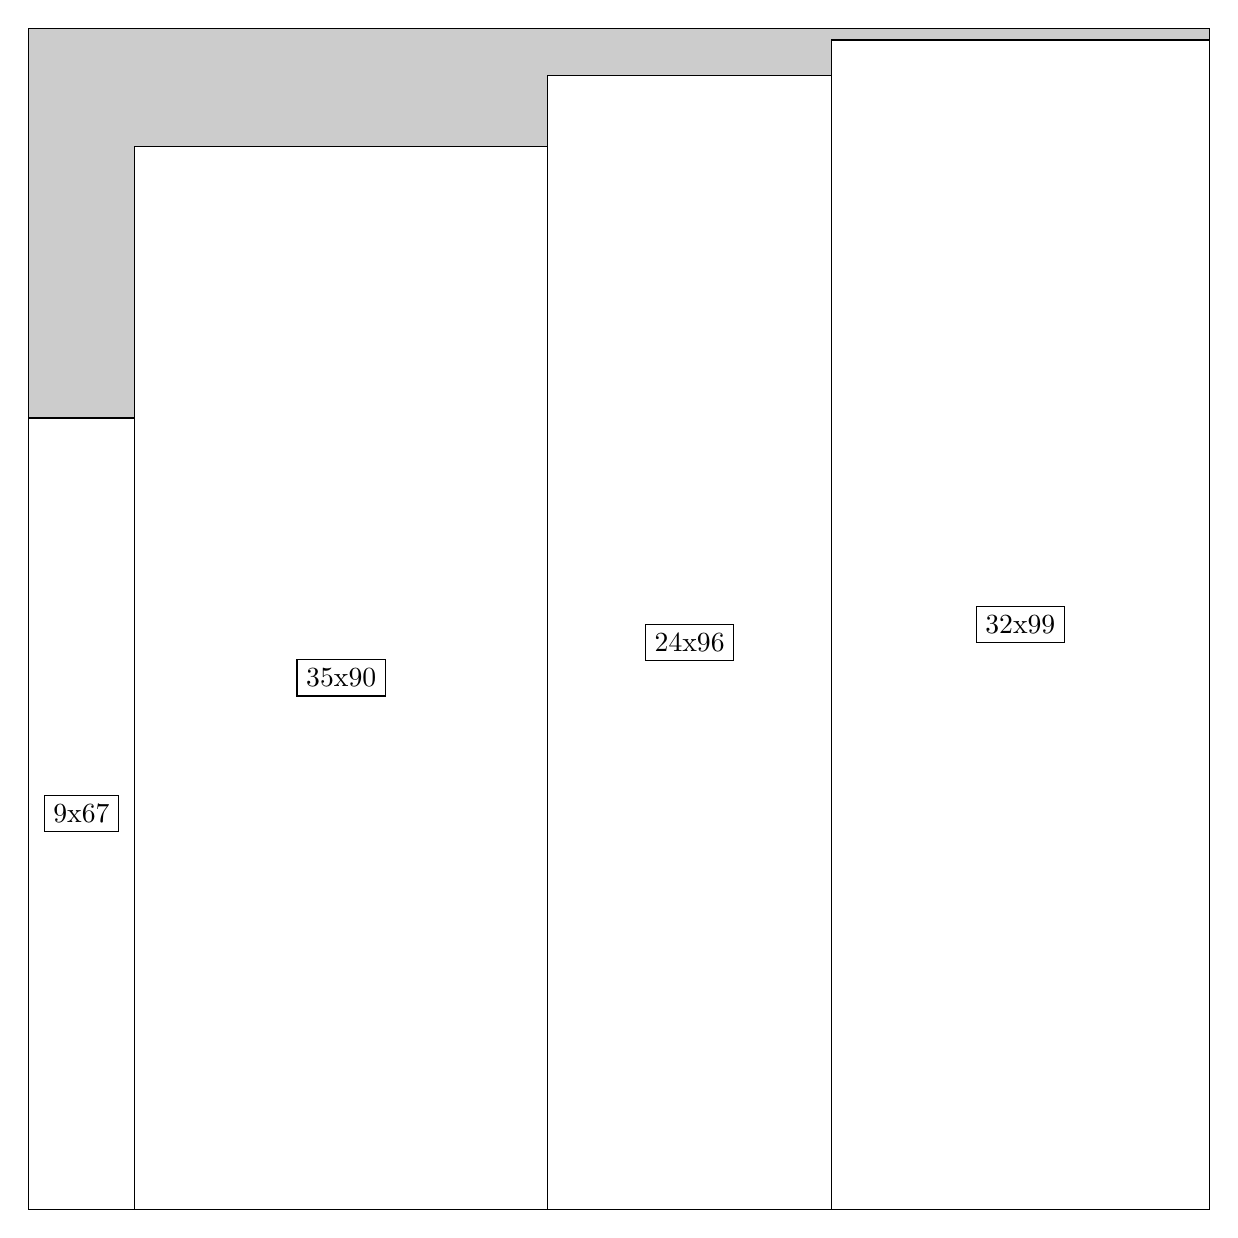
\begin{tikzpicture}[shorten >=1pt,scale=1.0,every node/.style={scale=1.0},->]
\tikzstyle{vertex}=[circle,fill=black!25,minimum size=14pt,inner sep=0pt]
\filldraw[fill=gray!40!white, draw=black] (0,0) rectangle (15.0,15.0);
\foreach \name/\x/\y/\w/\h in {32x99/10.2/0.0/4.8/14.85,24x96/6.6/0.0/3.5999999999999996/14.399999999999999,35x90/1.3499999999999999/0.0/5.25/13.5,9x67/0.0/0.0/1.3499999999999999/10.049999999999999}
\filldraw[fill=white!40!white, draw=black] (\x,\y) rectangle node[draw] (\name) {\name} ++(\w,\h);
\end{tikzpicture}


w =32 , h =99 , x =68 , y =0 , v =3168
\par
w =24 , h =96 , x =44 , y =0 , v =2304
\par
w =35 , h =90 , x =9 , y =0 , v =3150
\par
w =9 , h =67 , x =0 , y =0 , v =603
\par
\newpage


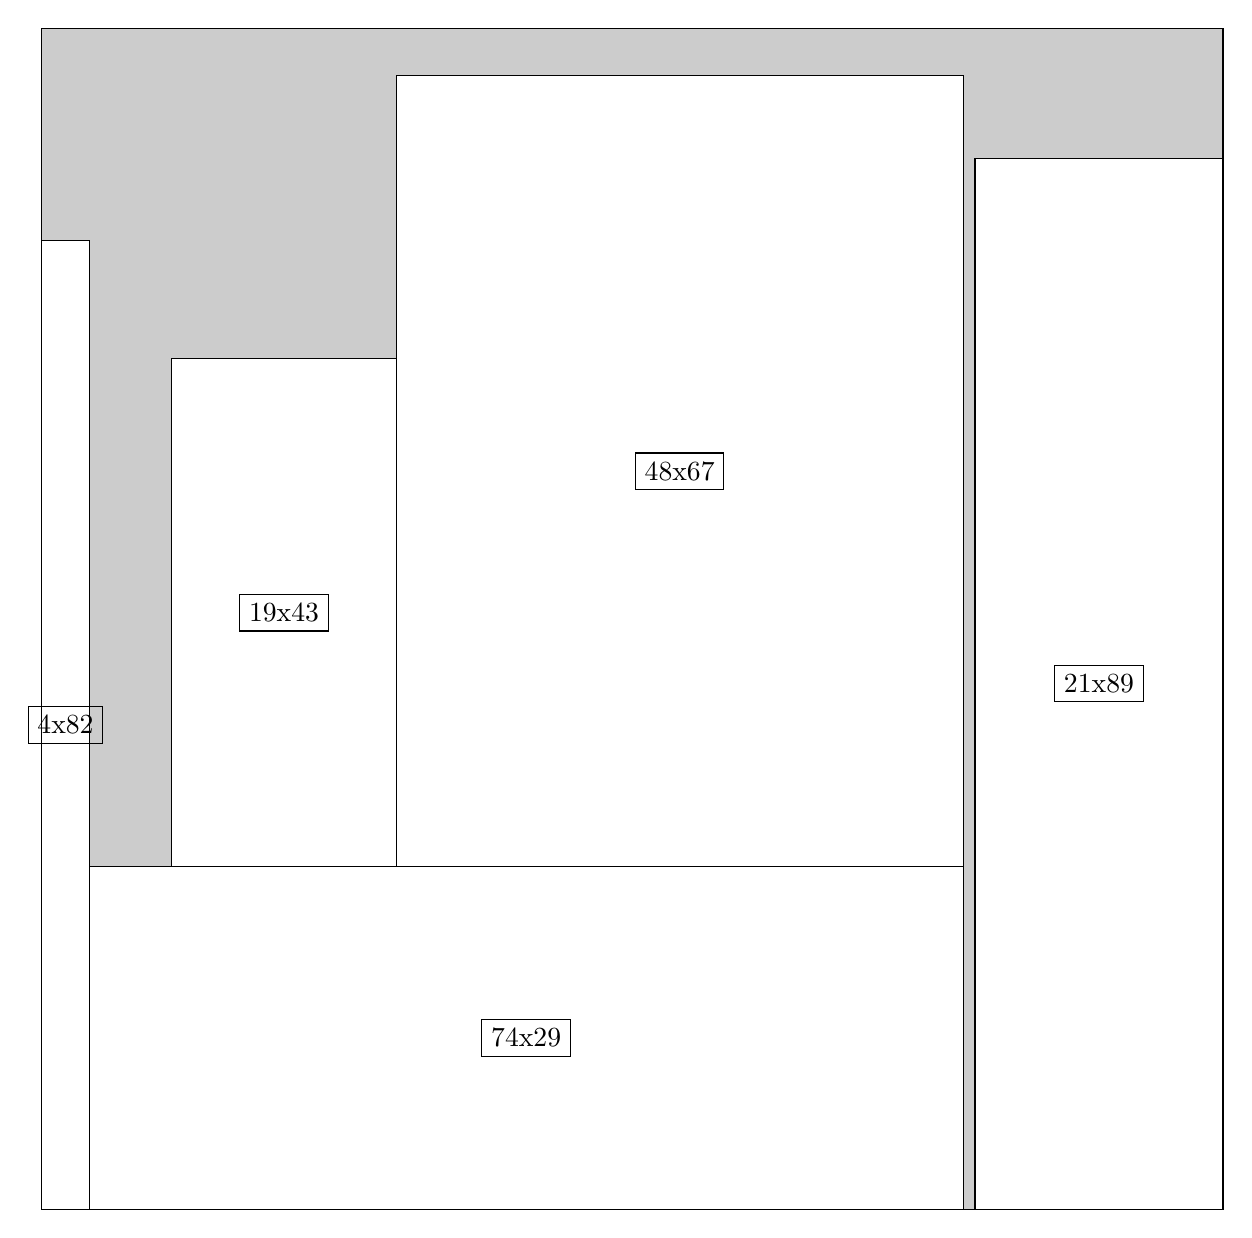
\begin{tikzpicture}[shorten >=1pt,scale=1.0,every node/.style={scale=1.0},->]
\tikzstyle{vertex}=[circle,fill=black!25,minimum size=14pt,inner sep=0pt]
\filldraw[fill=gray!40!white, draw=black] (0,0) rectangle (15.0,15.0);
\foreach \name/\x/\y/\w/\h in {21x89/11.85/0.0/3.15/13.35,74x29/0.6/0.0/11.1/4.35,48x67/4.5/4.35/7.199999999999999/10.049999999999999,19x43/1.65/4.35/2.85/6.45,4x82/0.0/0.0/0.6/12.299999999999999}
\filldraw[fill=white!40!white, draw=black] (\x,\y) rectangle node[draw] (\name) {\name} ++(\w,\h);
\end{tikzpicture}


w =21 , h =89 , x =79 , y =0 , v =1869
\par
w =74 , h =29 , x =4 , y =0 , v =2146
\par
w =48 , h =67 , x =30 , y =29 , v =3216
\par
w =19 , h =43 , x =11 , y =29 , v =817
\par
w =4 , h =82 , x =0 , y =0 , v =328
\par
\newpage


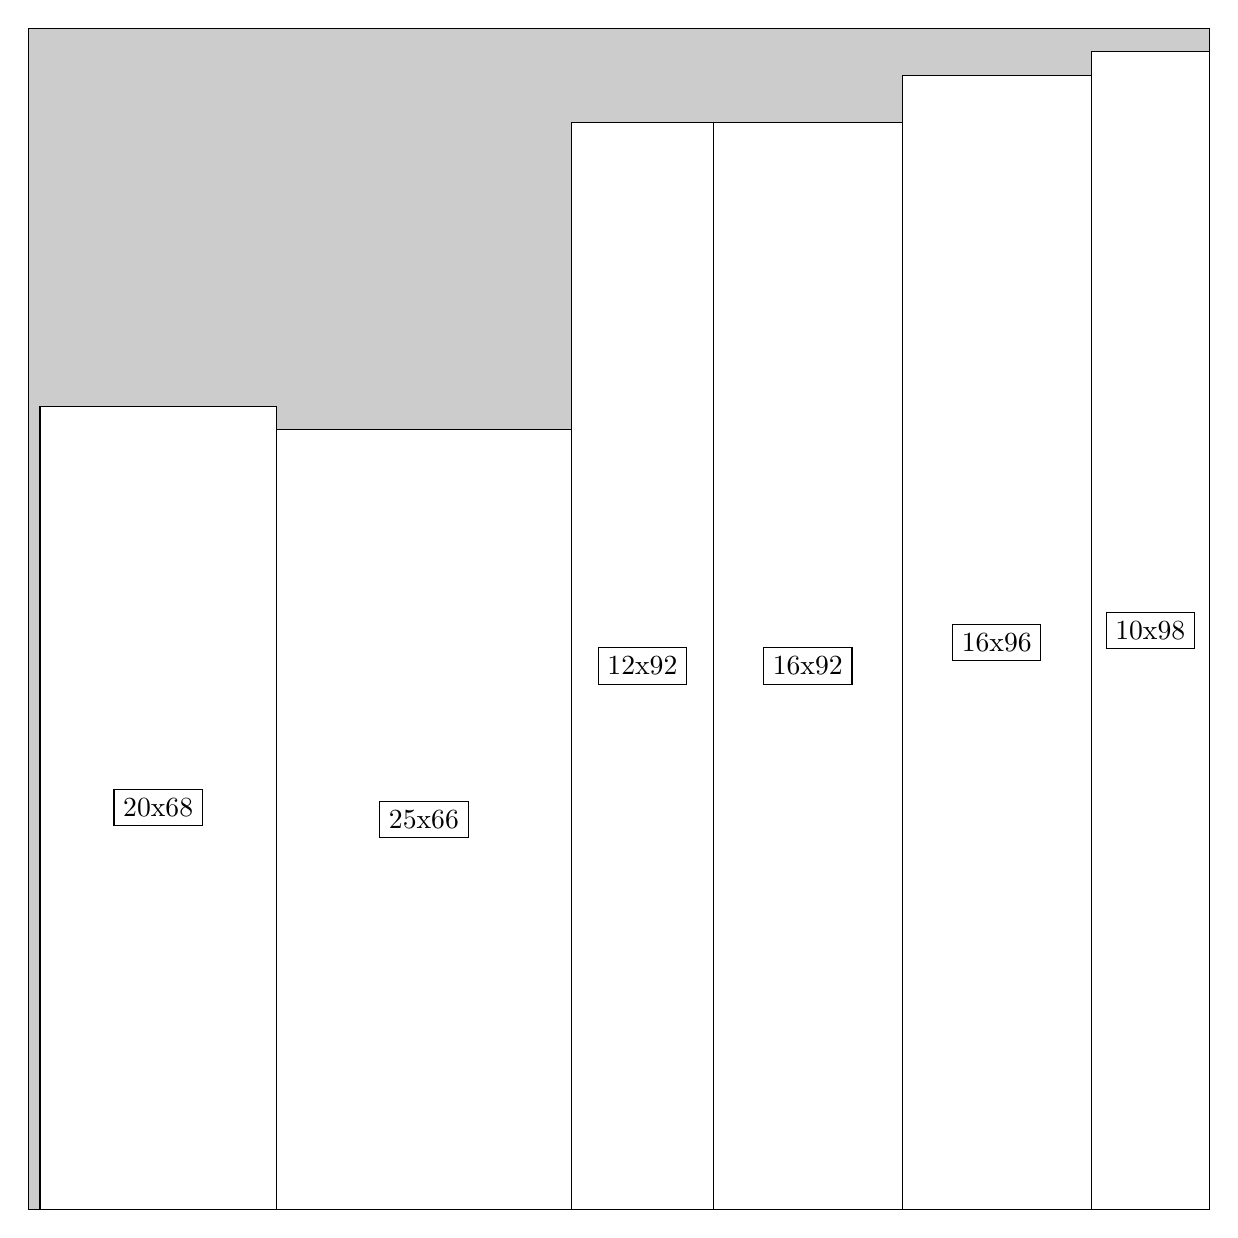
\begin{tikzpicture}[shorten >=1pt,scale=1.0,every node/.style={scale=1.0},->]
\tikzstyle{vertex}=[circle,fill=black!25,minimum size=14pt,inner sep=0pt]
\filldraw[fill=gray!40!white, draw=black] (0,0) rectangle (15.0,15.0);
\foreach \name/\x/\y/\w/\h in {10x98/13.5/0.0/1.5/14.7,16x96/11.1/0.0/2.4/14.399999999999999,16x92/8.7/0.0/2.4/13.799999999999999,12x92/6.8999999999999995/0.0/1.7999999999999998/13.799999999999999,25x66/3.15/0.0/3.75/9.9,20x68/0.15/0.0/3.0/10.2}
\filldraw[fill=white!40!white, draw=black] (\x,\y) rectangle node[draw] (\name) {\name} ++(\w,\h);
\end{tikzpicture}


w =10 , h =98 , x =90 , y =0 , v =980
\par
w =16 , h =96 , x =74 , y =0 , v =1536
\par
w =16 , h =92 , x =58 , y =0 , v =1472
\par
w =12 , h =92 , x =46 , y =0 , v =1104
\par
w =25 , h =66 , x =21 , y =0 , v =1650
\par
w =20 , h =68 , x =1 , y =0 , v =1360
\par
\newpage


\end{document}